\documentclass{article}
\usepackage[a4paper, total={6in, 8in}]{geometry}
\usepackage{amsfonts} 
\usepackage{graphicx}
\newcommand{\R}{\mathbb{R}}
\newcommand{\mrm}[1]{\mathrm{#1}}
\title{Multicriteria Optimization and Decision Analysis (MODA)\\ Assignment 1, 2022}
\author{Michael Emmerich (LIACS, Course Instructor),\\ Ksenia Pereverdieva (LIACS, Teaching Assistant), \\
Kamand Hajiaghapour (LIACS, Teaching Assistant)}
\begin{document}
	\maketitle
		This assignment is a graded homework. 
		%Parts will be graded in equal proportions (each 25\%).
	Assignment 1 covers the parts of the lecture that are important for the analytical ('mathematical') solution of multicriteria optimization problems. The computational solution will be covered in Assignment 2 (to be announced later). 
	\bigskip
	
\fbox{
\begin{minipage}{\textwidth}
\textit{\textbf{Submission (please read carefully)}: 
	Please upload your solution as a single PDF file with filename 
	$$MODA22A1\_\mbox{SNr1}\_Name1\_SNr2\_Name2\_SNr3\_Name3.pdf,$$ with SNr$=$ Studentnumber, via brightspace (as specified in the announcement). Clearly indicate your name(s) and student number(s) in the title and start a new page for each part (1-4) and clearly indicate the parts you are solving. }
\end{minipage}}
\medskip

\newpage
	\section{Linear Programming (\textit{20\%})}
	Let us define the following task:
	A paper factory wants to mix two ingredients, recycled pulp and pulp made of wood pulp.
	The variable $x_1$ is the amount(in $\mathrm{kg}$) of the first ingredient (recycled pulp) and the variable $x_2$ is the amount (in $\mathrm{kg}$) of the second ingredient (wood pulp).
	\begin{itemize}
	\item The profit achieved with a mixture is based on the cost of the ingredients and cost of cleaning and preprocessing. It has been estimated as $2 x_1 + 3 x_2$ and it should be maximized. 
	\item The cost per unit wood pulp is $2$ $ \mrm{Euro}$. 
	\item Recycled pulp has $0.5\mrm{g}/\mathrm{kg}$ water per unit, whereas wood pulp $1\mathrm{g}/\mrm{kg}$ water per unit. The total amount of water should not exceed $12 \mathrm{g}$ in a single charge.
	\item Recycled pulp has $2 \mathrm{g}/\mrm{kg}$ sulfur per unit, whereas wood pulp $1 \mathrm{g}/\mrm{kg}$ sulfur per unit. The total amount of sulfur should not exceed $14 \mrm{g}$ in a single charge.
	\item Recycled pulp has $6\%$ non-cellulose per unit, whereas wood pulp $2\%$ non-cellulose per unit. The total ratio of non-cellulose should not exceed $4\%$ in a single charge for raw material mix that enters the process.
    \end{itemize}
	\begin{eqnarray}
		2 x_1 + 3 x_2   &\rightarrow& \max\\
		0.5 x_1  +  x_2 &\leq& 12\\
		2 x_1 + x_2     &\leq& 14\\
		0.06 x_1 + 0.02 x_2   &\leq& 0.04(x_1 + x_2) 
	\end{eqnarray}
    \begin{itemize}
    	\item[Q1.1:]   Solve the problem of maximizing the profit of a charge graphically. Determine the maximum and the maximizer and draw all constraint boundaries in a diagram.
    	\item[Q1.2:] How would the problem solution change if $x_1$ and $x_2$ were integer variables, that is it is only possible to buy 0kg, or 1kg, or 2kg, or 3kg, $...$ of a raw material.
    	\item[Q1.3] Now, consider a second objective function, which is to maximize the amount of recycled pulp (to improve the environmental footprint). Determine graphically the efficient set and the Pareto front.
    	\item[Q1.4] Formulate the Karush Kuhn Tucker conditions for this problem and show that they hold in the optimal solutions.
    \end{itemize}

\newpage    
\section{Order Relations and Cones (\textit{20\%})}
In this part the goal is to investigate the properties of three different order relations. 
The first order relation is the $k$-dominance, defined as follows:
A vector $x \in \R^m$ is said to dominate a vector $y \in \R^m$ if and only if $x$ is better in more components than $y$. In other words we count in how many cases $x_i < y_i$ and in how many cases $y_i < x_i$ for all $i=1, ..., m$.
\begin{itemize}
	\item[Q2.1] Show that this order is equivalent to the Pareto order for $m=2$. Investigate, whether or not this order also defines a poset on $\R^3$ by considering the three axioms of a poset, and check whether they hold. 
	\item[Q2.2] Next consider the cone order for the cone ($C=\{\mathbf{y} \in \mathbb{R}| \mathbf{y} = u (0,1) + v (1,1) \ , u\geq 0, v\geq 0\}$). (a) Visualize the cone. (b) Investigate, whether the cone is pointed and convex. (c) Analyse whether or not the cone order  $x \preceq y \Leftrightarrow y \in x \oplus C$ is a partial order on $\mathbb{R}^2$ by checking whether the relevant axioms hold; and (d) draw the Hasse diagram for the set $\{(0,0), (1,1), (-1,1), (2,2), (-2,2), (0,2), (-1,2), (1,2)\}$.
	Remark: Note, the interesting fact that the cone is closely related to the Minkowski time-space cone (see lecture), but for movement in only one direction. 
%	\item[Q2.3] Investigate the following 'tolerant' indifference relation. $x \preceq y$, iff $x \leq y - \delta$. 
%	Show whether this order relation is transitive, (a) for $\delta > 0$, and (b) for $\delta < 0$. Also investigate whether the indifference relation $x \sim y \Leftrightarrow x\preceq_\epsilon y \wedge y \preceq_\epsilon x$ is transitive.  \\
%	Remark: Note, that the result will show a phenomenon called the 'intransitivity of indifference', that is the phenomenon that we do not notice change in every particular step, if change comes in small steps, but after a long series of small steps the overall change might become significant. (e.g. rising of the sea level in climate change, or gradual increase of prices).
\end{itemize}
\newpage
\section{Formulating Optimization Problems (\textit{30\%})}
Formulate the following problems in the modeling framework of mathematical programming, that is in the format:
$$f(x_1, \dots, x_r, z_1, \dots, z_s) \rightarrow \min$$
$$g_i (x_1, \dots, x_r, z_1, \dots, z_s), i=1, \dots, q$$
$$h_j (x_1, \dots, x_r, z_1, \dots, z_s), j=1, \dots, \ell$$
$$x_1, \dots, x_r\in \mathbb{R}$$
$$z_1, \dots, z_s\in \mathbb{Z}$$
Whenever possible, try to use linear and if that is not possible, quadratic objectives and constraints.

\begin{itemize}
\item[Q3.1] First formulate the problem of placing $k$ equally sized balls in a big sphere. Here $k$ is a constant and the radius of the balls has to be maximized. The big sphere has the radius of $10\mrm{m}$. A ball is defined by its center, that is $(x_i, y_i, z_i)$ for the i-th ball. Balls are not allowed to overlap and must be fully contained in the big sphere.
\item[Q3.2] Secondly formulate the problem of placing as many equally sized balls as possible in a big sphere.  The balls have the radius of $1 \mrm{m}$ and
the big sphere has the radius of $10\mrm{m}$.\\ 
Hint: Instead of looking at the Euclidean distances, it is useful to look instead at a formulation that uses squared Euclidean distances.
\item[Q3.3] Timetable: 
Let us assume we need to make a timetable for schools. Formulate this as a system of linear constraints on integer or binary variables. For doing so, use variables $x_{ijk} \in \{0,1\}$ and let $x_{ijk}$ equal to $1$ if subject $i$ is taught on day $j$ to hour $k$, and equal to $0$ otherwise.
\begin{enumerate}
	\item The school-week has $6$ days (Sunday is free).
	\item On day $1$ to day $5$ there are $6$ hours (timeslots), on day $6$ there are only $4$ hours (timeslots).
	\item There are the following subjects to be taught. (1) Maths, (2) English, (3) Dutch, (4) Geography, (5) Sports, (6) Music, (7) Arts, (8) Religion \& Ethics, (9) History, and (10) Science. Subjects 1, 2, and 3 are taught 6 hours per week, wheras subjects 4-10 are taught only 2 hours per week.
	\item There are four classes taught in parallel tracks: Classroom $1$, Classroom $2$, and Classroom $3$, and Classroom $4$. There is only one sports hall, and classrooms where music can be taught. For all the other classes there are no constraints. Each class is taught by the same class teacher, excepting music. For music there is only one teacher available at the school (and hence there can be only one music class at the same timeslot).
	\item The schedule should be such that each day the same subject is taught at most two times.  
	\item When a subject is taught on one day, there should be a break of one day before it is taught again. Sunday counts as a break.
	\item Besides the constraints, there is a score function which rewards Maths, English, and Dutch  being taught in earlier hours and math to be taught at later hours of the day. The score function is given by $\sum_{i=1}^3\sum_{k=1}^{L_j} \sum_{j=1}^6 k^2 x_{ijk} + \sum_{k=1}^{L_j} \sum_{j=1}^6 (L_j-k)^2 x_{5jk}$. (to decide whether it needs to be minimized or maximized is part of the task).
\end{enumerate}
\end{itemize}

\newpage
\section{Analytical Solution of Multiobjective Optimization Problem (\textit{30\%})}
Consider the task of minimizing a the surface area of a prism given 
by 
$$S(a,h)= 2 ah + \sqrt{2} ah + a^2 $$
while maximizing its volume
$$V(a,h)= \frac{1}{2} a^2 h, $$
$$a,h \geq 0.$$
\begin{figure}[t]
	\begin{center}
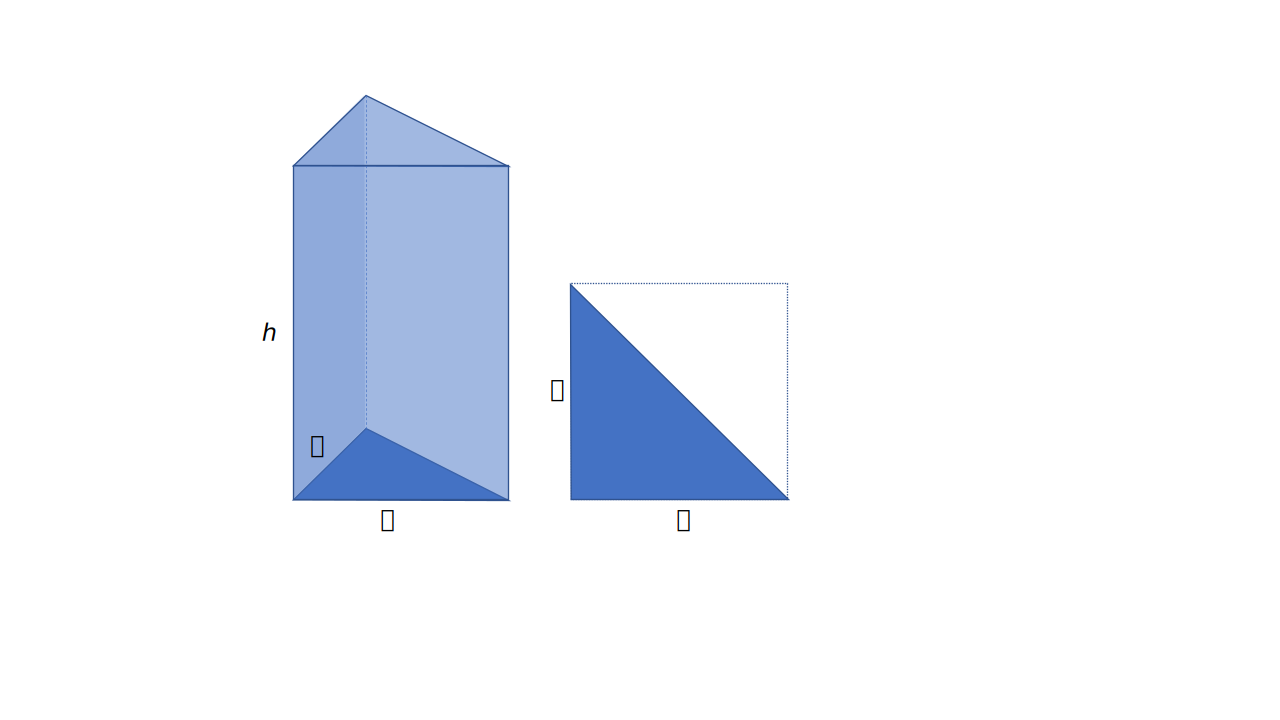
\includegraphics[width=10cm]{prism2022}
	\end{center}
\end{figure}
\begin{itemize}
	\item[Q4.1:] (\textit{20\%}) First, consider $V$ to be constant (equality constraint $V(a,h) - V_{epsilon} = 0$ for some constant $V_{\epsilon} > 0$. Solve the constraint optimization problem with the Lagrange multiplier rule.
	\item[Q4.2:] (\textit{10\%}) Secondly, derive the efficient set of the problem of minimizing the surface area $f_1(a,h)$ and maximizing the volume ($f_2(a,h)$) using the $\epsilon$-constraint methods (using equality constraints to scan the efficient set). Provide a mathematical expression of the Pareto front in the form of a parameterized curve (form: $\{ \mathbf{x} \in \mathbb{R}^2 | \mathbf{x}=(u(a,h,V_{\epsilon}), h(a,h, V_{\epsilon}))  \})$ and an expression of the Pareto front as a function.
	\item[Q4.3 ] (\textit{10\% Bonus question}\footnote{By answering correctly the bonus question you can compensate for points lost in other parts of the assignment.}) Draw the level curves (contours) of V(a,h) and of S(a,h) in a 2-D contour plot and indicate graphically the Pareto front. You can for instance use python-matplotlib or wxMaxima for doing so and include the picture in your report. Hint: You can use the graphical solution to double check the result obtained in with 4.2. 
\end{itemize}

End of Assignment 1 (MODA 2022) -- \textit{Wishing you Success!}
\end{document}